%==============================================================================
% PREAMBLE
%==============================================================================
\documentclass[mathserif, xcolor=dvipsnames]{beamer}
% \usepackage{helvet}
\usepackage[T1]{fontenc}
\usepackage{amsmath, amsfonts,amsthm}
\usepackage{url}
\usepackage{listings}
\lstset{basicstyle=\ttfamily\footnotesize}
\usepackage{color}

\usetheme[height=10mm]{Rochester}
\usecolortheme[named=MidnightBlue]{structure}
\setbeamertemplate{navigation symbols}{}

\title{Git primer}
\author{Vincent Dumoulin}
\date{January 15, 2015}

%==============================================================================
% BODY
%==============================================================================
\begin{document}

%------------------------------------------------------------------------------
% TITLE
%------------------------------------------------------------------------------
\begin{frame}[plain]
    \titlepage
\end{frame}

%------------------------------------------------------------------------------
% Why version control?
%------------------------------------------------------------------------------
\begin{frame}
    \frametitle{Why version control?}
    \begin{itemize} \addtolength{\itemsep}{0.5\baselineskip}
        \item{A nice and clean alternative to maintaining multiple versions of
              the same file using some sort of custom naming scheme
              (\emph{e.g.} \texttt{myfile\_9.py})}
        \item{A way to end the fear of saving and quitting}
        \item{Keep a trace how your files change throughout development}
        \item{Revert back to older versions}
        \item{Manage multiple versions (\emph{branches}) of your code at the
              same time}
        \item{For more information, see
              \url{http://git-scm.com/book/en/v2/Getting-Started-About-Version-Control}}
    \end{itemize}
\end{frame}

%------------------------------------------------------------------------------
% What is git?
%------------------------------------------------------------------------------
\begin{frame}
    \frametitle{What is git?}
    \begin{itemize}\addtolength{\itemsep}{0.5\baselineskip}
        \item{Distributed version control system
              \begin{itemize}
                  \item{No checking out single files: local version fully
                        mirrors the repository}
                  \item{No central authority on what is the \emph{true}
                        codebase}
               \end{itemize}}
        \item{Takes \emph{snapshots} of the state of a repository at a given
              time}
        \item{Intelligent about not duplicating information from one snapshot
              to another}
        \item{For more information, see
              \url{http://git-scm.com/book/en/v2/Getting-Started-Git-Basics}}
    \end{itemize}
\end{frame}

%------------------------------------------------------------------------------
% What is Github?
%------------------------------------------------------------------------------
\begin{frame}
    \frametitle{What is Github?}
    \begin{itemize}\addtolength{\itemsep}{0.5\baselineskip}
        \item{A place to host your git repositories}
        \item{Makes it easy to
              \begin{itemize}
                  \item{Share code with others}
                  \item{Keep track of other people's code}
                  \item{Modify other people's code (\emph{forking})}
                  \item{Collaborate with other people on common code}
              \end{itemize}}
        \item{Technically no different from your own machine:
              \begin{itemize}
                  \item{Both can pull and push changes}
                  \item{Both host a fully functional version of your repository}
              \end{itemize}}
    \end{itemize}
\end{frame}

%------------------------------------------------------------------------------
% Basic workflow using git and Github
%------------------------------------------------------------------------------
\begin{frame}
    \frametitle{Git + Github workflow: repo creation}
    \begin{figure}[H]
        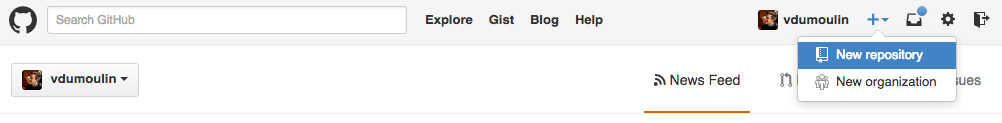
\includegraphics[width=\textwidth]{repo_creation_1.png}
    \end{figure}
\end{frame}

\begin{frame}
    \frametitle{Git + Github workflow: repo creation}
    \begin{figure}[H]
        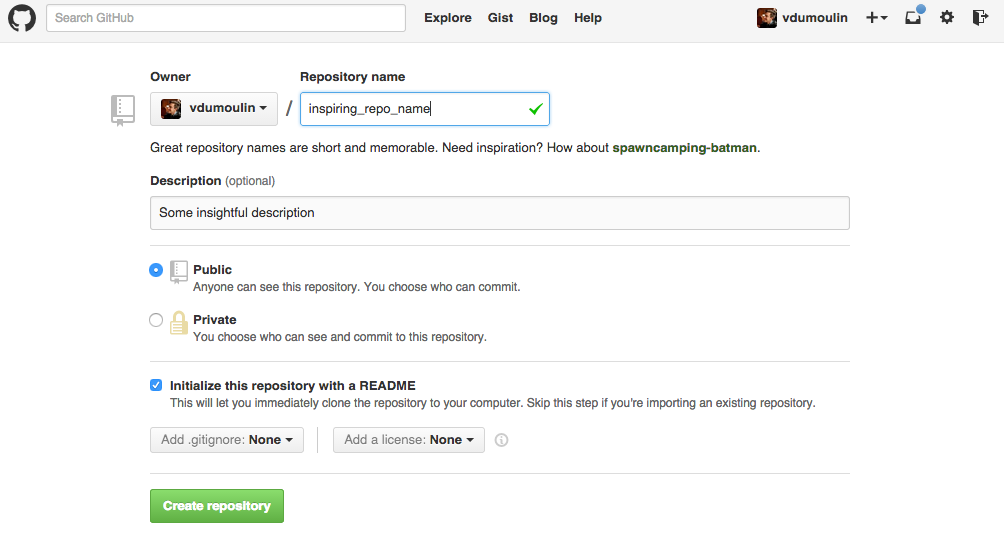
\includegraphics[width=\textwidth]{repo_creation_2.png}
    \end{figure}
\end{frame}

\begin{frame}[fragile]
    \frametitle{Git + Github workflow: repo cloning}
    \begin{figure}[H]
        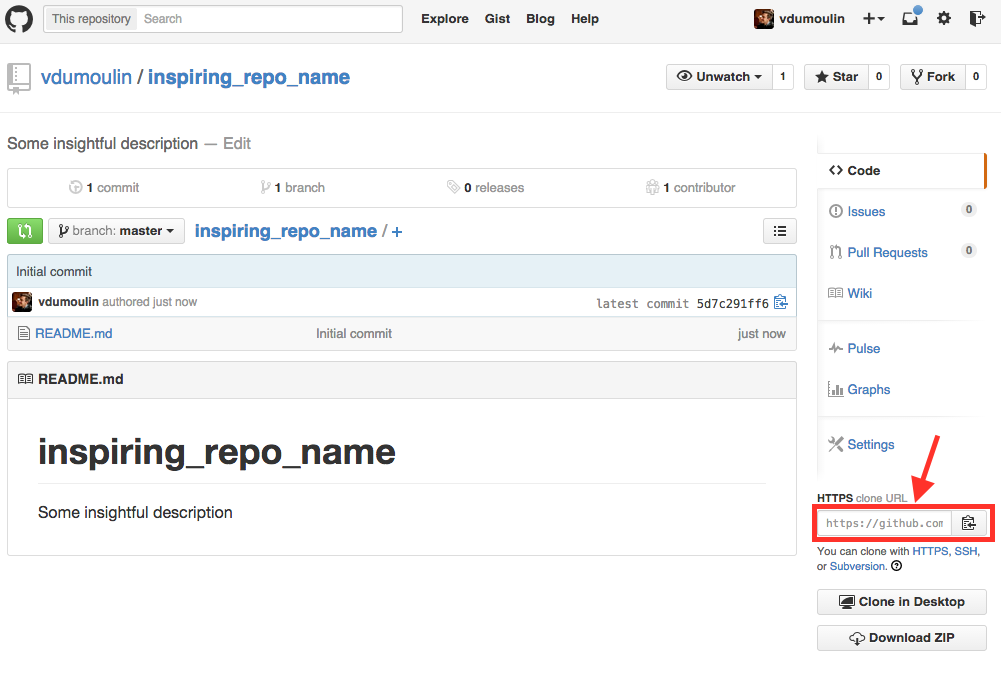
\includegraphics[width=0.8\textwidth]{repo_cloning.png}
    \end{figure}
\begin{lstlisting}
> git clone \
    https://github.com/vdumoulin/inspiring_repo_name.git
\end{lstlisting}
\end{frame}

\begin{frame}[fragile]
    \frametitle{Git + Github workflow: put a file under version control}
    \begin{itemize}
        \item{Create a dummy file:
\begin{lstlisting}
> echo 'print "This is file A"' > file_a.py
\end{lstlisting}}
    \item{Check the status of the repo:
\begin{lstlisting}
> git status
[...]
Untracked files:
  (use "git add <file>..." to include in what [...]

        file_a.py
nothing added to commit but untracked files [...]
\end{lstlisting}}
        \item{Add the file to version control:
\begin{lstlisting}
> git add file_a.py
\end{lstlisting}}
        \item{Commit the newly-added file:
\begin{lstlisting}
> git commit -m "Add file_a.py to repository"
[master a82a245] Add file_a.py to repository
 1 file changed, 1 insertion(+)
 create mode 100644 file_a.py
\end{lstlisting}}
    \end{itemize}
\end{frame}

\begin{frame}[fragile]
    \frametitle{Git + Github workflow: commit changes to a file}
    \begin{itemize}
        \item{Change something in your file:
\begin{lstlisting}
> echo 'print "It is pretty useless"' >> file_a.py
\end{lstlisting}}
        \item{Stage the changes:
\begin{lstlisting}
> git add file_a.py
\end{lstlisting}}
        \item{Commit the changes:
\begin{lstlisting}
> git commit -m "Add useful line to file_a.py"
\end{lstlisting}}
    \end{itemize}
\end{frame}

\begin{frame}[fragile]
    \frametitle{Git + Github workflow: push changes on Github}
    \begin{itemize}
        \item{First, pull the latest changes from your Github repo:
\begin{lstlisting}
> git pull origin master
\end{lstlisting}}
        \item{Push your changes to Github:
\begin{lstlisting}
> git push origin master
\end{lstlisting}}
    \end{itemize}
\end{frame}

%------------------------------------------------------------------------------
% For more information
%------------------------------------------------------------------------------
\begin{frame}
    \frametitle{Going further}
    For more information, have a look at this very complete git reference:
    \begin{center}
        \url{http://git-scm.com/book/en/v2}
    \end{center}
\end{frame}

\end{document}
